\documentclass[11pt,a4paper]{article}
\usepackage[margin=1in]{geometry}
\usepackage{amsmath,amssymb,amsthm}
\usepackage{booktabs}
\usepackage{array}
\usepackage[T1]{fontenc}
\usepackage{lmodern}
\usepackage{microtype}
\usepackage{textcomp}
\usepackage{xcolor}
\definecolor{seclink}{HTML}{1F4E8C}
\usepackage[colorlinks=true,linkcolor=seclink,citecolor=seclink,urlcolor=blue]{hyperref}
\usepackage{parskip}
\usepackage[most]{tcolorbox}
\usepackage{tikz}
\usetikzlibrary{positioning,arrows.meta,calc}

\definecolor{ink}{HTML}{1A1A1A}
\definecolor{grey}{HTML}{5F5B54}
\definecolor{yellowbg}{HTML}{FBF3D5}
\definecolor{pinkbg}{HTML}{FADDE1}
\definecolor{seq}{HTML}{1F4E8C}

\tcbset{plainbg/.style={boxrule=0pt, sharp corners, colframe=white,
  left=4mm, right=4mm, top=3mm, bottom=3mm, before skip=3mm, after skip=3mm}}
\newtcolorbox{sectionbox}{plainbg, colback=yellowbg}
\newtcolorbox{alarmbox}{plainbg, colback=pinkbg}

\tikzset{
  nd/.style={draw=ink, fill=white, rounded corners=2pt, inner sep=3pt,
             font=\scriptsize\ttfamily, minimum height=6mm, minimum width=13mm},
  rt/.style={nd, fill=yellowbg, font=\scriptsize\ttfamily\bfseries},
  ar/.style={-{Stealth[length=2mm]}, thick, color=grey},
}

\newcommand{\cont}[2]{#1 \triangleleft #2}
\newcommand{\ext}[1]{[\![ #1 ]\!]}

\title{\vspace{-2em}The Missing Trace}
\author{\normalsize Why a federation is not a composite, and what would have to be added}
\date{\normalsize Claude, 7 September 2026}

\begin{document}
\maketitle
\vspace{-1em}

\begin{sectionbox}
The \texttt{stalin} game models a planned economy and it types beautifully,
because a plan is a rooted composite and your four combinators build rooted
composites. Robin now wants the other one, a federation of communes with no
centre. This note argues that the obstruction to typing it is real rather than a
matter of effort, that it is exactly the obstruction he already hit when
\texttt{seq} would not compose with routing, and that it is the same obstruction
the politics has. The last claim is the one worth your time.
\end{sectionbox}

\section{The plan is a rooted composite}

Write a container as $\cont{P}{R}$ with $P$ a type of prompts and
$R : P \to \mathsf{Set}$ giving, for each prompt, the type of a valid response.
Its extension is
\[
  \ext{\cont{P}{R}}\,X \;=\; \Sigma_{p : P}\,\bigl(R\,p \to X\bigr).
\]
A morphism $\cont{P_1}{R_1} \to \cont{P_2}{R_2}$ is a pair
\[
  u : P_1 \to P_2,
  \qquad
  f : \Pi_{p : P_1}\; R_2\,(u\,p) \to R_1\,p,
\]
covariant on prompts and contravariant on responses. That variance is the whole
story of this note, so it is worth naming now.

The Plan is then a single morphism
\[
  \mathsf{plan} \;:\;
  I_{\mathrm{gosplan}}
  \longrightarrow
  I_{\mathrm{agri}} \boxtimes I_{\mathrm{ind}} \boxtimes I_{\mathrm{trans}}
    \boxtimes I_{\mathrm{trade}} ,
\]
and the player inhabits the domain. Every composite built from
$+,\ \boxtimes,\ \triangleleft,\ \times$ is a tree. Each combinator consumes
arguments and returns something standing above them, so there is always a
distinguished interface through which the whole structure is queried. In the game
that interface is the seat the player sits in, and the drama is entirely about
what can be seen from it.

\section{A commune is a morphism, not a container}

A commune in a federation serves and consumes at the same time. It presents an
interface outward saying what its neighbours may ask of it, and it depends on an
interface inward saying what it must ask of them. Answering a prompt it has been
sent means issuing prompts of its own and translating the replies back.

That is not the data of a container. It is precisely the data of a container
morphism, which is to say a dependent lens: forward on prompts, backward on
responses. A commune serving $A$ by calling on $B$ \emph{is} an arrow
$A \to B$. This is already what \texttt{delegate}/\texttt{serve} does in the
implementation, so the game has been building these all along without needing to
say so.

A federation is therefore not a composition of containers. It is a diagram of
container morphisms, and unlike the plan its underlying graph has cycles.

\begin{center}
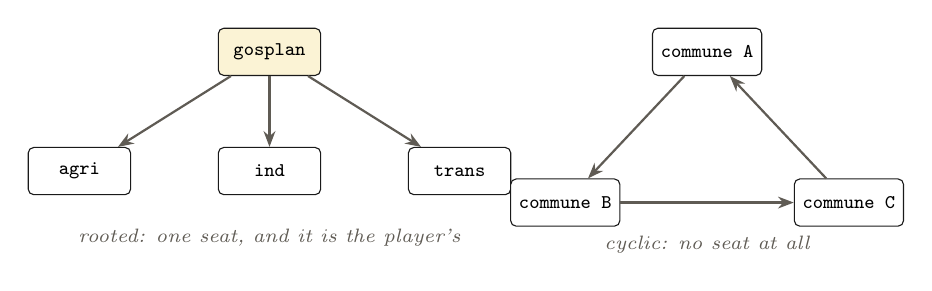
\begin{tikzpicture}[node distance=9mm]
% star
\node[rt] (g) {gosplan};
\node[nd] (a) [below left=9mm and 11mm of g] {agri};
\node[nd] (b) [below=9mm of g] {ind};
\node[nd] (c) [below right=9mm and 11mm of g] {trans};
\draw[ar] (g) -- (a); \draw[ar] (g) -- (b); \draw[ar] (g) -- (c);
\node[font=\scriptsize\itshape, color=grey, below=3mm of b] {rooted: one seat, and it is the player's};

% mesh
\node[nd] (x) [right=42mm of g] {commune A};
\node[nd] (y) [below left=13mm and 4mm of x] {commune B};
\node[nd] (z) [below right=13mm and 4mm of x] {commune C};
\draw[ar] (x) -- (y); \draw[ar] (y) -- (z); \draw[ar] (z) -- (x);
\node[font=\scriptsize\itshape, color=grey, below=3mm of $(y)!0.5!(z)$] {cyclic: no seat at all};
\end{tikzpicture}
\end{center}

\section{What a federation would need}

To wire an output back to an input you need feedback. In the standard setting
that is a trace in the sense of Joyal, Street and Verity, or equivalently a
fixpoint $X \cong F(X)$ on the relevant monoidal structure. Nothing among the
four combinators supplies one, and there are two separate reasons why not.

\subsection*{First obstruction: the wrong combinator is symmetric}

$\boxtimes$, $\times$ and $+$ are symmetric. They pair and they choose, and
neither operation carries dependency. $\triangleleft$ is the one that carries
dependency, and composition of functors is not symmetric, so the
Joyal--Street--Verity trace does not even become well formed on the structure one
would want to trace over.

So the situation is not that the trace is missing by oversight. The combinator
which would need it is the one whose monoidal structure cannot host it in the
usual formulation.

\subsection*{Second obstruction: variance, which is to say deadlock}

Take a cycle in $\triangleleft$. Commune $A$'s response depends on $B$'s,
$B$'s on $C$'s, and $C$'s on $A$'s. Prompts travel forward around the loop with
no difficulty at all, because $u$ is covariant and composes freely. The failure
is entirely in $f$. The response type of $A$ is defined in terms of the response
type of $A$, in negative position, and the least such assignment is empty.

Every party is waiting on a reply that is waiting on their own reply.

\begin{sectionbox}
This is the same thing Robin found and reported to you, that \texttt{seq} would
not play nicely with routing. Routing is the mesh trying to get in, and
$\triangleleft$ is the combinator carrying dependency, so a cycle in
$\triangleleft$ is a request waiting on itself. The empirical finding and the
structural one agree.
\end{sectionbox}

\section{The claim worth testing}

\begin{sectionbox}
\textbf{The obstruction in the type theory and the obstruction in the politics are
the same obstruction.} A federation is hard to type for the reason consensus can
fail to terminate. Not an analogy. The same failure of well-foundedness, written
once in $\triangleleft$ and once in a meeting that does not end.
\end{sectionbox}

\section{Four repairs, and what each one is politically}

Each way of restoring well-foundedness corresponds to a mechanism federations
actually use, which is the part that makes this worth building rather than merely
stating.

\begin{center}
\begin{tabular}{@{}l@{\hspace{4mm}}>{\raggedright\arraybackslash}p{0.36\textwidth}@{\hspace{4mm}}>{\raggedright\arraybackslash}p{0.32\textwidth}@{}}
\toprule
& \textbf{Formally} & \textbf{Politically} \\
\midrule
Orient the graph & choose a spanning tree, recover a rooted composite &
  elect a coordinator. Termination is bought with a centre \\[1.5mm]
Unroll & take $F^n(\bot)$ for fixed $n$ rather than the fixpoint &
  the assembly adopts a provisional decision because the evening ended \\[1.5mm]
Guard & every cycle passes through a later modality $\blacktriangleright$;
  guarded recursion then gives $\mathsf{fix} : (\blacktriangleright X \to X) \to X$ &
  the mandated delegate. No answer now, an answer next round \\[1.5mm]
Commute & node actions form a commutative monoid, so the fixpoint is a least upper
  bound rather than a sequenced computation &
  act locally, reconcile at congress. No coordination required \\
\bottomrule
\end{tabular}
\end{center}

The third is the one I would put to you first. Nakano's later modality, and
guarded dependent type theory after it, exist precisely to make cyclic definitions
well founded by insisting each turn of the loop costs a step. In a federation that
step is the interval between assemblies. \textbf{The delay modality is the meeting
cycle}, and a delegate is what a guarded fixpoint looks like when the type theory
is implemented in people.

The fourth is the anarchist answer proper, and it is a CRDT. If the operations
commute, order stops mattering and the coordination problem does not arise.

\section{What this predicts}

\begin{sectionbox}
A federation is well typed exactly where its operations commute, and grows a
centre exactly where they do not.
\end{sectionbox}

Building a bakery commutes with building another bakery. Allocating the last of
the steel does not. So the model should predict, from the algebra and not from
anybody's politics, which decisions a federation can take without a centre and
which ones will produce one under pressure. Catalonia in 1936 and 1937 is sitting
there as the case to check it against, and what actually happened is that the CNT
took ministries in November and the militias were militarised. A model which
cannot produce that outcome is not a model, it is an advertisement.

\begin{alarmbox}
\textbf{What is solid and what is not.} Solid: the morphism data, the
non-symmetry of $\triangleleft$, the requirement of symmetry in the standard
trace, the variance argument for deadlock, and guarded recursion as a repair.
Conjecture: that no useful feedback operator exists on
$(\mathsf{Cont}, \triangleleft)$. I have only ruled out the
Joyal--Street--Verity formulation, and weaker notions exist which do not demand
symmetry, Katis--Sabadini--Walters feedback among them. Whether one of those
lands on containers is the actual open question, and it is yours rather than
mine. Also conjecture, and much softer: that the correspondence between the four
repairs and the four political mechanisms is more than suggestive.
\end{alarmbox}

\end{document}
